% !TEX root = migratedoc.tex
\chapter{Presentation of results}

\section{Maximum likelihood inference}
There are several differences between the \ma and \ba output. The outfput exists typically in two files
a textfile called outfile (default name) and a PDF called outfile.pdf, for changing these names consult the 
input/output menu. The maximum likelihood analsysi writes to a PDF file but because of time constraints
I never completely finished that transition (perhaps next year), therefore for \ma use the textfile as the main
output, EXCEPT if you are interested in the distribution of the migration and coalescence events through time,
that is only plotted into the PDF (see below).

Contents of the output in \texttt{ outfile}: Some of the output options vary
according to the datatype.  + = always present, o = optional, Default = $\star$
\newcommand{\st}{$\star$}
\smallskip
\begin{center}
\begin{tabular}{l p{10cm} c}
\hline
Item & Description  & Status\\
\hline
List of options & {all used options are specified} & +\\
Summary of data & {(Too) short data summary} & +\\
Dataset & Print of the dataset & o\\
MCMC estimates & {List of the estimated parameters for each locus and the mean} & +\\
Shape $\alpha$ & {Estimation of the shape parameters $\alpha$ for the variation of the mutation rate}  & o\\
\fst table & {Table of the possible start values generated with a \fst estimator}  & o \\
plots & {plot of the likelihood surface in outfile} & o\st \\
  & {plot of the likelihood surface into mathfile} & o\\
$\alpha$-histogram & {Table of shape values versus log(likelihood), $\alpha$ is varying whereas the other parameters are held constant at the maximum of the surface.} & o\\
Profiles & {Profile likelihood tables} & o\st \\
Percentiles & {Percentiles table, summary of profile tables} & o\st\\
Event histograms & {Distribution of events over time} & o\\
\hline 
\end{tabular}
\end{center}
The $F_{ST}$ calculations are based on mean differences in populations compared
to mean differences between populations, for more information you should consult \cite{maynardsmith:1970:psp, nei:1972:igd, beerli:1999:mle}, .

\subsection{Walk through an outfile}
The following output pieces are from \texttt{ outfile.seq} in the \texttt{ example} directory.
\subsubsection{Title and Options}
\begin{center}
\begin{boxedminipage}{6in}
\begin{footnotesize}
\ttfamily{
\begin{verbatim}
 =============================================
   An example with sequence data
 =============================================
  MIGRATION RATE AND POPULATION SIZE ESTIMATION
  using Markov Chain Monte Carlo simulation
  =============================================
  Version 2.0.3

  Program started at Sat Dec 18 19:56:23 2004
         finished at Sun Dec 19 01:22:31 2004
     
Options in use:
---------------
Datatype: DNA sequence data
Random number seed (with internal timer)           1103417783
Start parameters:
   Theta values were generated  from the FST-calculation
   M values were generated from the FST-calculation
Migration model:
   Migration matrix model with variable Theta  
Mutation rate is constant for all loci
Analysis strategy is                          Maximum likelihood
Markov chain settings:
   Short chains (short-chains):                           10
      Trees sampled (short-inc*samples):               20000
      Trees recorded (short-sample):                    1000
   Long chains (long-chains):                              3
      Trees sampled (long-inc*samples):               200000
      Trees recorded (long-sample):                    10000
   Averaging over replicates:                              2
   Static heating scheme
      4 chains with  temperatures
       1.00, 1.57, 2.71, 5.00
      Swapping interval is 1
   Number of discard trees per chain:                  10000
Print options:
   Data file:                               infile.check-mig
   Output file:                                      outfile
   Print data:                                            No
   Print genealogies:                                     No
   Plot data: Yes, to outfile and mathfile                  
              Parameter: {Theta, M}, Scale: Log10, Intervals: 36
              Ranges: X-    M: 0.000100 - 100.000000
              Ranges: Y-Theta: 0.000100 - 100.000000
   Profile likelihood: Yes, tables and summary             
             Percentile method
             with df=1 and for Theta and M=m/mu
\end{verbatim}
}
\end{footnotesize}
\end{boxedminipage}
\end{center}
This is the title and options part. Don't cut away the options, so you will 
still
know a few weeks later with what kind of options and how long you
run the program.
\newpage
\subsubsection{Summary of the data}
\begin{center}
\begin{boxedminipage}{6in}
\begin{small}
\ttfamily{
\begin{verbatim}
Summary of data:
---------------
Datatype:                                       Sequence data
Number of loci:                                             2

Population                                    Locus  Gene copies
----------------------------------------------------------------
  1 Tallahassee                                  1     20
                                                 2     20
  2 Sopchoppy                                    1     20
                                                 2     20
  3 St._George Island                            1     20
                                                 2     20
Total of all populations                         1     60
                                                 2     60


Empirical Base Frequencies
------------------------------------------------------------
Locus     Nucleotide                        Transition/
          ------------------------------  Transversion ratio
          A       C       G       T(U)
------------------------------------------------------------
   1      0.2515  0.2730  0.2283  0.2472       2.00000
   2      0.2465  0.2350  0.2627  0.2557       2.00000

\end{verbatim}
}
\end{small}
\end{boxedminipage}
\end{center}
The data summary is (too) short, and self explanatory, you can also print
the data (not shown). Print the data the first time you use the program with
your data and check if it was read correctly: I control the first and the last
individual in a population and check a few sites at both ends of the sequence.
If the program crashes shortly after the start, almost certainly the data
contains some trouble. The most common error is having the wrong number
of individuals and/or number of sites, or having miscounted the number of characters in the individual name.
\newpage
\subsubsection{Parameter estimates}
\begin{center}
\begin{boxedminipage}{6in}
\begin{small}
\ttfamily{
\begin{verbatim}
==============================================================================
MCMC estimates 
==============================================================================
Population [x] Loc.  Ln(L)   Theta    M [m/mu] [+=receiving population]  
                             [xNe mu]    1,+     2,+     3,+    
-------------- ---- -------- -------- ----------------------------------------
 1: Tallahasse  1 1   11.406  0.04326 ------- 22.9291  0.0000 
                1 2    0.875  0.04006 -------  0.0000  0.0000 
                1 A    1.754  0.04009 -------  0.0000  0.0000 
                2 1    2.463  0.03418 -------  0.0000 11.8760 
                2 2    3.246  0.04276 -------  4.1693 12.4264 
                2 A    4.158  0.04214 -------  3.8056 12.1477 
                All   20.696  0.04330 -------  8.6572  0.0000 
 2: Sopchoppy   1 1   11.406  0.01553  5.6584 -------  3.2363 
                1 2    0.875  0.01996 12.0396 -------  0.0000 
                1 A    1.754  0.01993 12.0679 -------  0.0000 
                2 1    2.463  0.00918  0.0000 ------- 14.9951 
                2 2    3.246  0.01485  0.0000 ------- 16.6994 
                2 A    4.158  0.01444  0.0000 ------- 16.5949 
                All   20.696  0.01283  0.0000 -------  2.0536 
 3: St._George  1 1   11.406  0.00969  0.0000  0.0000 -------
                1 2    0.875  0.01125  0.0000  5.8414 -------
                1 A    1.754  0.01124  0.0000  5.8325 -------
                2 1    2.463  0.01174 13.0240  0.0000 -------
                2 2    3.246  0.01025 20.5578  0.0000 -------
                2 A    4.158  0.01039 19.7503  0.0000 -------
                All   20.696  0.01088  3.4871  3.2021 -------

Comments:
 The x is 1, 2, or 4 for mtDNA, haploid, or diploid data, respectively
There were 10 short chains (1000 used trees out of sampled 20000)
  and 3 long chains (10000 used trees out of sampled 200000)
  Static heating with 4 chains was active
  COMBINATION OF 2 MULTIPLE RUNS)
\end{verbatim}
}
\end{small}
\end{boxedminipage}
\end{center}
This is the main output of the program. For each population there is a list
of all estimates for each locus and each replicate and their over-all-replicate and over-all-loci estimates. The replicate summary estimates are not simple averages but use a method devised by Geyer (1994: reverse logistic regression). The summary over loci is summing up the likelihood curves under the assumption that each locus is independent of the other (a rather save assumption as long one is not working with multiple mtDNA or Y-chromosome loci).
%\par
%The ln(L) is the maximum log likelihood.
%This value is a ratio $ln(L) = ln(L(\P)/L(\P_0))$ and is always above 0.0 in this table. The parameter $\P_0$ are
%different between different runs of the program and therefore you cannot
%simply compare between different runs.
%\par
%The column marked Theta ($\Theta$) gives the population sizes for 
%each population and each locus, of course the number of individuals
%in that population $N_e$ is for all loci the same, and the variance you see
%is (a)  the variance of the sampler, 
%(b) stochastic variance due to the coalescence
%process, (c) variance of the mutation rate.
%The migration parameter $\M$  table is to read the following way:
%in population 1, the \textbf{ 2,+} means that the immigration from population two into one is $\M_{21}=8.6572$.
%in population 2 the \textbf{ 1,+} means that the immigration from population one into two is $\M{12}=0.0000$
%If the program is also allowing for variable mutation rate (you don't want to
%use that with only few loci), then you will get also an estimate for the 
%shape parameter alpha ($\alpha$) for the distribution of the mutation rates.  
%
%\subsubsection{\fst table}
%This will be shown when print-fst=YES is set. If you want to use this you need to reread the appendix of Beerli and Felsenstein (1999). It is merely used as a starting 
%value for the Maximum likelihood estimates. The table are similar to the table
%of the MCMC estimates.

%\subsubsection{Likelihood surface plots}
%For each population and each locus there will be a summary contour plot
%for all immigrations and all 'emmigrations'. These plots give some information
%about the confidence you should have in the estimates. Keep in mind that
%even with two populations there are 4 parameters and the likelihood.
%A plot is a kind of diagonal through this high dimensional space (in this
%example: 10 dimensions). The contour plots in the \textbf{outfile} are very crude, but the contour data is also written into the \textbf{mathfile} and this can be displayed with programs such as mathematica (see example program earlier) or gnuplot and could look like the following contourplot, it is the same as the left graph shown on the next page. The graph shows the total immigration rates, expressed as $\M$ versus the population size $\Theta$.
%\begin{center}
%\begin{boxedminipage}{4in}
%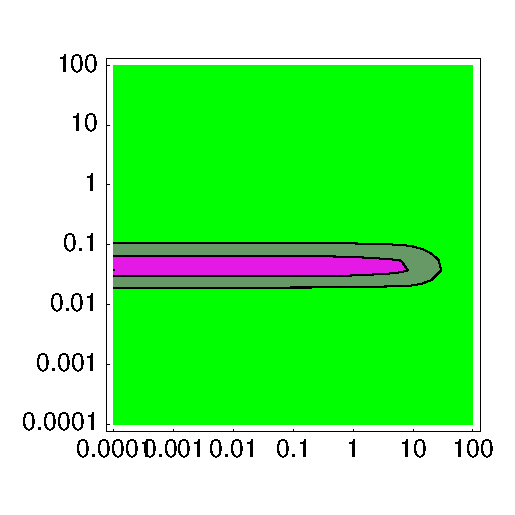
\includegraphics{mim/mathfilegraph}
%\end{boxedminipage}
%\end{center}
%\newpage
%\begin{center}
%\begin{boxedminipage}{6.5in}
%\begin{small}
%\ttfamily{
%\begin{verbatim}
%[the figure is edited so that it fits better on the page]
%n-Likelihood surfaces for each of the   3 populations
%-------------------------------------------------------
%
%Legend:
%   X = Maximum likelihood
%   * = in approximative 50% confidence limit
%   + = in approximative 95% confidence limit
%   - = in approximative 99% confidence limit
%X-tickmarks are (1) 0.000100, (2) 0.001585, (3) 0.025119
%                (4) 0.398107, (5) 6.309573, (6) 100.000000
%Y-tickmarks are (1) 0.000100, (2) 0.001585, (3) 0.025119
%                (4) 0.398107, (5) 6.309573, (6) 100.000000
%
%Over all loci
%
%    x-axis=   M [xNm = effective population size * migration rate = Theta * M
%                  M   = migration rate / mutation rate = m/mu],
%x=1, 2, or 4 for mtDNA, haploid, or diploid data
%    y-axis = Theta,
%    units = see above
%Population 1: population__number___0
%  **Average** immigration: M=0.000100, Theta=0.037276, log likelihood=20.332327
%  **Average** emigration: M=1.930698, Theta=0.037276, log likelihood=20.769244
%[Remember: the maximum values are from a grid]
%
%          Mean(Immigration)                       Mean(Emigration)
%
%      1      2      3      4      5      6      1      2      3      4      5      6
%     ++------+------+------+------+------++    ++------+------+------+------+------++
%   6 +                                    +    +                                    +
%     |                                    |    |                                    |
%     |                                    |    |                                    |
%   5 +                                    +    +                                    +
%     |                                    |    |                                    |
%     |                                    |    |                                    |
%   4 +                                    +    +                                    +
%     |                                    |    |                                    |
%     |                                    |    |                                    |
%     |                                    |    |                                    |
%     |++++++++++++++++++++++++++++++-     |    |+++++++++++++++++++++++++++++++--   |
%     |******************************++    |    |********************************++  |
%     |X******************************+-   |    |*************************X*******+- |
%   3 ++++++++++++++++++++++++++++++++-    +    ++++++++++++++++++++++++++++++++++-  +
%     |                                    |    |                                    |
%     |                                    |    |                                    |
%     |                                    |    |                                    |
%     |                                    |    |                                    |
%   2 +                                    +    +                                    +
%     |                                    |    |                                    |
%     |                                    |    |                                    |
%   1 +                                    +    +                                    +
%     ++------+------+------+------+------++    ++------+------+------+------+------++   
%      1      2      3      4      5      6      1      2      3      4      5      6
%
%\end{verbatim}
%}
%\end{small}
%\end{boxedminipage}
%\end{center}
%\subsubsection{Likelihood ratio tests}
%The likelihood ratio test printout consists of a legend that explains the likelihood ratio tables and the tables themselves. the lefts side states the hyopthesis and the right side shows the associated values.
%\begin{center}
%\begin{boxedminipage}{6in}
%\begin{small}
%\ttfamily{
%\begin{verbatim}
%==============================================================================
%Likelihood ratio tests
%==============================================================================
%Over all loci
%Legend for the LRT tables
%-------------------------------------------------------------------------------
%Null-Hypothesis: your test model         | Log(likelihood) of test model
%=same=                                   | Log(likelihood) of full model
%full model (the model under which the    | Likelihood ratio test value
%genealogies were sampled)                | Degrees of freedom of test
%[Theta values are on the diagonal of the | Probability*
%Migration matrix, migration rates are    | Probability**
%specified as M]                          | Akaike's Information Criterion***
%                                         | Number of parameters used
%-------------------------------------------------------------------------------
%  *) Probability under the assumption that parameters have range -Inf to Inf
% **) Probability under the assumption that parameters have range 0 to Inf
%***) AIC: the smaller the value the better the model
%          [the full model has AIC=1125.401453, num(param)=9]
%-------------------------------------------------------------------------------
%H0: 0.0458 5.8386 5.3308 5.8386 0.0169 2.1822 5.33 | LnL(test) = -1606.113074
%    2.1822 0.0103                                  | LNL(full) = -553.700726
% =  0.0458 9.4132 0.0000 2.2639 0.0169 4.3644 10.6 | LRT       = 2104.824696
%    0.0000 0.0103                                  | df        = 6
%[ *, s, s, s, *, s, s, s, *,]                      | Prob      = 0.000000
%                                                   | Probc     = 0.000000
%                                                   | AIC       = 3226.226148
%                                                   | num(param)= 7
%-------------------------------------------------------------------------------
%\end{verbatim}
%}
%\end{small}
%\end{boxedminipage}
%\end{center}
%\newpage
%\subsubsection{Profile likelihoods}
%\begin{center}
%\begin{boxedminipage}{6in}
%\begin{small}
%\ttfamily{
%\begin{verbatim}
%Profile likelihood for parameter Theta_1
%Parameters are evaluated at percentiles.
%-------------------------------------------------------------------------------
%Per.  Ln(L)     Theta_1     *Theta_1*   Theta_2     M_21       M_12      
%-------------------------------------------------------------------------------
%0.01  -3.645      0.0223     0.0223     0.0297    81.9303   293.8230 
%0.05  -2.065      0.0240     0.0240     0.0297    81.9441   294.2779 
%0.10  -1.329      0.0250     0.0250     0.0297    81.9766   294.5011 
%0.25  -0.284      0.0266     0.0266     0.0296    82.0709   294.7953 
%0.50   2.878*     0.0457     0.0457     0.0286    88.4385   273.2104 
%0.75   0.324      0.0789     0.0789     0.0279    96.2738   252.5011 
%0.90  -1.065      0.0900     0.0900     0.0277    97.4555   251.1683 
%0.95  -1.910      0.0966     0.0966     0.0277    98.0544   250.5631 
%0.99  -3.884      0.1119     0.1119     0.0276    99.2213   249.4557 
%-------------------------------------------------------------------------------
%\end{verbatim}
%}
%\end{small}
%\end{boxedminipage}
%\end{center}
%
%The profile likelihood table show how the parameters vary
%when we hold one parameter constant. In the default setting the program tries to
%find the parameter values that are at the percentiles.
%How is this done for $\Theta_1$:
% calculate the likelihood value for
%\begin{enumerate}
%  \item a few values smaller and bigger than the ML-estimate. 
%  \item calculate a spline
%function. 
%\item find the $\Theta_1$ that is at the percentile $x$ using the
%splines. 
%\item recalculate the likelihood and maximize the other parameter again
%using the full formula.
%\end{enumerate} 
% In the example, $\Theta_1$ varies almost independently from the others, but looking more closely it seems that $\Theta_2$ slightly
%shrinks while $\Theta_1$ grows.
%
%Sometimes, the algorithm to find the percentiles fails, in this case  the program prints instead of the precentile values \texttt{***} and warns that it failed to calculate the percentiles. The calculates likelihoods and parameter values are still correct but simply not at the percentile values. Earlier versions of the program did not tell the user about this shortcoming.
%\newpage
%\subsubsection{Summary of profile likelihood tables}
%\begin{center}
%\begin{boxedminipage}{6in}
%\begin{small}
%\ttfamily{
%\begin{verbatim}
%===============================================================================
%Summary of profile likelihood percentiles of all parameters
%===============================================================================
%
%Parameter                          Lower percentiles
%            -------------------------------------------------------------------
%                0.01          0.05          0.10          0.25          0.50
%-------------------------------------------------------------------------------
%Theta_1         0.02228       0.02399       0.02497       0.02664       0.04567
%Theta_2         0.00946       0.01188       0.01331       0.01567       0.02857
% M_21          30.53718      36.49126      39.97529      46.64759      88.43845
% M_12         114.08445     132.49441     143.22648     163.32323     273.21045
%
%
%Parameter                          Upper percentiles
%            -------------------------------------------------------------------
%                0.50          0.75          0.90          0.95          0.99
%-------------------------------------------------------------------------------
%Theta_1         0.04567       0.07889       0.09003       0.09660       0.11190
%Theta_2         0.02857       0.05709       0.07586       0.09833       0.15052
% M_21          88.43845     201.06595     215.26333     225.18048     245.85767
% M_12         273.21045     805.85153     896.08361     957.07762    1083.66503
%-------------------------------------------------------------------------------
%\end{verbatim}
%}
%\end{small}
%\end{boxedminipage}
%\end{center}
%
%This summarizes only the likelihood and profile parameter column from the
%profile likelihood tables and can be used to give some idea about the 
%confidence you should have into the estimates.
%$\Theta_1$ has a \textbf{approximative} 90\%-confidence interval from 0.02399 to 0.09660
%with a best estimate of 0.04567.
%(the data was simulated with a $\Theta_1=0.05$.
%If the percentile calculation failed, this summary plot needs to be evaluated carefully, the program warns about possible problems by printing an \texttt{*} next to then value in question.
%\newpage

\section{Bayesian inference}

\subsection{Walk through an outfile}

The main output of a Bayesian run contains of the following table that summarizes the posterior distribution and an acceptance ratio table. The table of the posterior distribution is characterized for each locus and each parameter and percentiles, median, mode, and mean. The posterior distribution over all loci is also presented graphically (Figure \ref{BAYESTABLEHIST}). 

\begin{figure}[htb]
\begin{center}
\includegraphics[scale=0.6]{mim/bayestable}\\
\includegraphics[scale=0.6]{mim/bayeshist}
\end{center}
\caption{Table and Figure example of a Bayesian posterior distribution. \label{BAYESTABLEHIST}}
\end{figure}


%The acceptance ratio tables give some idea whether the Markov chains has mixed and explored many different values.
%\begin{center}
%\begin{boxedminipage}{6in}
%\begin{small}
%\ttfamily{
%\begin{verbatim}
%Bayesian estimates
%==================

%Locus Parameter  2.5%      25.0%   median    75.0%   97.5%     mode     mean
%-----------------------------------------------------------------------------
%    1  Theta_1   0.00986  0.00434  0.00932  0.00000  0.07356  0.00602  0.01272
%    1  Theta_2   0.00439  0.00171  0.00372  0.00000  0.06915  0.00274  0.00448
%    1  M_2->1        644   614.46   623.20     0.00  3654.57   189.32   872.45
%    1  M_1->2        197   197.11   193.09     0.00  6890.91     4.02   369.93

%

%Acceptance ratios for all parameters and the genealogies (Locus 1
%---------------------------------------------------------------------

%Parameter           Accepted changes            Ratio
%Theta_1                 90646/125195            0.72404
%Theta_2                 61965/125195            0.49495
%M_2->1                  80238/125194            0.64091
%M_1->2                  63487/125194            0.50711
%Genealogies             22270/500000            0.04454
%\end{verbatim}
%}
%\end{small}
%\end{boxedminipage}
%\end{center}
% plot of a credibility set etc
\newpage
\section{Histograms over time}
\subsection{Events through time}
\migrate allows to investigate the pattern of events through time, the histograms represent the frequency of recorded events during the MCMC run, the location of these events in time are determined by the data (that is what we want to see) but depends on the length of runs, and how well the genealogies were explored (that is what we want to have no influence!). \migrate is assuming the all the events in every time units come from the same prior distribution (BA) or driving value (MA). For simulated data from populations that are constant in size through time and that exchange migrants at a constant rate, we expect distributions that look similar exponential decay. If either the data was generated by a process that is not constant through time the histogram will look different (figure \ref{MIGPROBHIST}). The time is measure in unites of generation / mutation rate per generation (and site) .
\begin{figure}[htb]
\begin{center}
\includegraphics[scale=0.8]{mim/frequencyM}
\end{center}
\caption{Frequency of migration events between between two populations through time. Today is left on the graph; units are generation per mutation rate 
\label{MIGPROB}}
\end{figure}
\migrate also prints out tables that report average time for migration and coalescence events for all events and for the most recent common ancestors, and that supplies the probability in which population the sample originated (Figure \ref{MIGPROBTABLE}). This seem to work fine with equal sample sizes , but may be skewed with unequal sample size (for example for two populations: 100 and 10). Unequal sizes may need much longer run time to say some thin with confidence. In addition, a single locus may not give really relevant results, use multiple loci if you can.
\begin{figure}[htb]
\begin{center}
\includegraphics[width=8cm]{mim/sumfreq}
\includegraphics[width=8cm]{mim/timeMRCA}
\end{center}
\caption{Left: Tables of frequencies and average time for all events. Right: Table of the probability of the location of the most recent common ancestor. \label{MIGPROB}}
\end{figure}

\subsection{Skyline plots}

\begin{figure}[!h]
\begin{center}
\includegraphics[scale=0.9]{mim/skylineTheta}\\

\includegraphics[scale=0.9]{mim/skylineM}
\end{center}
\vskip -1cm 
\caption{Skyline plot of a population that recently increased strongly , the time is in units of mutation-scaled generations. Top: population size, bottom: one example immigration rate into the population shown on top.
\label{SKYPLOT}}
\end{figure}

\migrate has its own version of skyline plots \cite{strimmer:2001:edh,Shapiro:2004:RFB,Drummond:2005:bci}. \migrate reports averages and standard deviation of expected parameter values calculated from the genealogy. The proposal for all timeintervals uses the constant population size and migration rate, so it is different from  \cite{Drummond:2005:bci} and certainly needs more evaluations. \migrate can summarize over multiple loci, take into account several data types, and reports the parameters changes through time also for migration parameters. \migrate has several short-comings: for example it assumes that the mutation rate is constant per locus, which make affect results for some data sets, but because \migrate is typically used for populations within species or very closely related species, I hope that the mutation rate of a specific locus will not change considerably.

A legend for these plots is printed toward the end:
\begin{footnotesize}
\begin{verbatim}
Skyline plots: 
Skyline plots visualize the changes of population sizes and migration rates through time 
(today is on the left side and time is measured into the past. The time scale is in units of 
expected mutations per generation. To calculate the absolute time scale you must supply an 
mutation rate per year and the duration of a  generation in years in the data option. 
You can calculate the absolute time by multiplying the scale by generation time times 
mutation rate per year (per site for DNA; per locus for all other datatypes). 
With estimated mutation rate only the combined rate modifier is plotted. 
[this will change to  mutation rate plot]. 
The gray bars cover one approximate standard deviation up and down from the expected value. 
The bar with different shades of gray on top of each plot indicates the number of values that were used 
to calculate the expected value, white means there are very few and black means. 
that there were man thousands of samples per bin. 
On some plots one can see red squares below the grayscale bar, these suggest that either the 
upper quantile and/or the main value was higher than the visible part of the  axis. 
Event histograms: 
All accepted events (migration events, coalescent events) are recorded and their frequency 
are shown as histograms over time with recent time on the left side. The frequency plots of 
populations with constant size and constant immigration rates show histograms that are similar 
to exponential distribution, if the populations come from a divergence model without migration 
then the frequency of migration events can show a peak in the past.
\end{verbatim}
\end{footnotesize}
\chapter{Output that is not part of the outfile}
\migrate writes the raw data that is used to generate the histograms and tables in the PDF and the textfile into several files, such as the \textsl{bayesfile}, \textsl{bayesallfile}, \textsl{mighistfile} and the \textsl{skylinefile}. Each file contains a header that gives you some idea what the values mean and you can process these files by yourself using graphing programs (or \tracer). I highlight here a use of the the print-tree option.
 
\section{Potential genealogy plots}
\migrate allows to record the best genealogy visited in the course of the MCMC run, this treefile contains migration events and currently only the program \texttt{ eventtree} (ET) (Palczewski and Beerli unpubl. -- popgen.scs.fsu/et ) can plot these events. Remember this is not necessarily the best possible tree for the data, but the most likely visited tree, in tests with small dataset we could show that with real species tree \migrate recovers the topology, but because it does not optimize branch length, will make errors on the length of the branches, it also assumes a clock.
\begin{figure}[bh]
\centering \includegraphics[width=10cm]{mim/human_tree}
\caption{Best visited genealogy of a 3 population run with Neanderthals, modern humans, and chimpanzees. The arrows on the tree mark migration events --  there is very little power to pinpoint these migration events and the events shown are a haphazard sample of many possible migration events that happen to occur on the topology that is most compatible with the data, The color was added using Adobe Illustrator.\label{MIGTREE}}
\end{figure}

\newpage
\chapter{Diagnostics}
\migrate prints out several diagnostics, these diagnostics are not sufficient to judge whether your data was run successfully, but you should run the program minimally two times to compare the results and not trust the diagnostics. The acceptance/rejection ratios for all parameters (BA) and the genealogy (MA, BA) give some idea about how many new parameters or trees are in the MCMC sample, if the ration is very low the autocorrelation will be high and the effective sample size of trees and parameters will be low. For MA a statistic described by Gelman and Rubin \cite{kass:1998:mcm} can be used to get some idea about convergence. The Gelman-Rubin statistic is broken for some of the analysis option, but I believe that multiple runs from different start settings (different start parameter and random tree) are a great way to explore the behavior of the MCMC run(s).

The last page of the output can contain  \textbf{ Warnings} that suggest whether some parameters did not converge or not (Figure \ref{ESS}). 
\begin{figure}[bh]
\begin{center}
\includegraphics[width=8cm]{mim/acceptance}
\includegraphics[width=8cm]{mim/ess}
\includegraphics[width=8cm]{mim/warnings}
\end{center}
\caption{Acceptance Ratios, Effective sample size and autocorrelation, and Warnings of a run.
\label{ESS}}
\end{figure}

\newpage
